\chapter[Resultados]{Resultados}

Neste capítulo, serão apresentados os principais resultados obtidos usando uma abordagem híbrida quantitativa e qualitativa, conduzida com cenários de uso e pesquisa-ação. Este capítulo apresenta dados referentes ao desenvolvimento da prova de conceito e do próprio simulador, que são considerados resultados deste trabalho. As subseções "Testes Unitários e Cobertura de Código" e "Métricas de Qualidade de Código" apresentam dados obtidos através de um levantamento quantitativo visando uma análise qualitativa do código fonte do simulador desenvolvido. Por fim, foi realizada análise dos cenários de uso levantados.

\section{Prova de conceito}

A fim de entender melhor o domínio da aplicação e verificar a viabilidade do projeto, foi desenvolvida uma prova de conceito. Essa prova de conceito permitiu que alguns elementos que não puderam ser identificados apenas na fase inicial do projeto com o referencial bibliográfico estudado, fossem identificados, podendo assim, compor uma proposta mais refinada da solução. 

\subsection{Especificações técnicas}

As especificações técnicas da máquina, a qual foi utilizada para a realização do desenvolvimento da prova de conceito foram, um processador Intel Core i7, modelo 2630QM de 2Ghz e uma memória RAM de 6Gb. O sistema operacional utilizado foi o Ubuntu, versão 14.10 de 64 bits.

\subsection{Descrição da prova de conceito}

Para a construção dos agentes, optou-se pelo uso do \textit{framework} JADE. O principal motivo desta escolha foi o fato de ser uma ferramenta reconhecida pela comunidade que trabalha com sistemas multiagentes, e por seguir os padrões e normas estabelecidos pela FIPA\footnote{\url{http://www.fipa.org/}}. Outro fator que foi levado em consideração na escolha do \textit{framework} foi o fato de ser uma plataforma estabilizada no processo de criação de agentes além da sua boa documentação. \cite{franca}. O JADE é inteiramente implementado na linguagem de programação JAVA, portanto, as aplicações que fazem uso deste \textit{framework} assim como sua integração com o mesmo, orientam-se por meio dessa linguagem. 

Com base na literatura estudada, identificamos alguns elementos físicos importantes, candidatos a serem representados no sistema. Esses foram representados de forma simples para esta prova de conceito, tais como: paredes, obstáculos e fontes sonoras. Esses elementos físicos são utilizados para compor o ambiente a ser representado dentro do sistema. O som também deve ser representado, porém, o conceito de onda sonora foi substituído pelo de raio sonoro. O som representado como raio sonoro pode ser entendido como retas dirigidas segundo a direção em que as mesmas caminham, permitindo assim, tratar melhor o evento da reflexão sonora \cite{silva}. O conceito de raio sonoro já é utilizado por grande parte dos produtos de software na área de simulação acústica.

A princípio, todos os elementos identificados foram tratados e implementados como agentes de software. O ambiente foi desenvolvido como o agente principal, responsável pela criação de todos os outros agentes, os quais, ao final, acabam por compor a estrutura do ambiente, com exceção do som, que deve ser criado pela fonte sonora dentro do sistema.

Esse modelo apresentou alguns problemas de desempenho, no qual tornou inviável o uso de um volume maior de agentes. Portanto, um novo modelo foi proposto. O modelo consiste em uma solução híbrida, composta pelos paradigmas multiagentes e orientado a objetos, onde os obstáculos do ambiente são tratados como objetos, devido ao fato de não terem um papel significativo na comunicação dos agentes, pois são elementos estáticos dentro do sistema. Os demais elementos como o ambiente, a fonte sonora e o som se mantiveram como agentes de software, sendo o ambiente responsável por agrupar os demais elementos do sistema, que são, fontes sonoras (agentes) e obstáculos (objetos). 

A fonte sonora é o agente responsável pela criação dos sons, simulando o comportamento de pulso sonoro. Já os sons, são os agentes mais ativos dentro do projeto, sendo responsáveis por exercerem seu papel e percorrerem todo o ambiente, identificando as devidas colisões, reflexões e alterando seus parâmetros de intensidade sonora, direção, dentre outros, até que o mesmo atinja uma intensidade inaudível, ocasionando assim o fim do mesmo.

O agente som, dentro do sistema, é tratado como um ponto dentro do mapa do ambiente. A fonte sonora é o agente responsável pela criação desses agentes sonoros, emitindo assim um arco com uma abertura de acordo com a configuração da fonte. Por exemplo, caso uma fonte sonora tenha sido configurada para emitir um pulso sonoro com uma abertura de 90º e os agentes sonoros sejam criados com um intervalo de um grau, essa fonte sonora irá lançar 91 agentes sonoros a partir de sua origem, que no caso será a fonte sonora. A figura \ref{fonte_sonora} ilustra esse evento.
 
\FloatBarrier 
\begin{figure}[!htb]
\centering
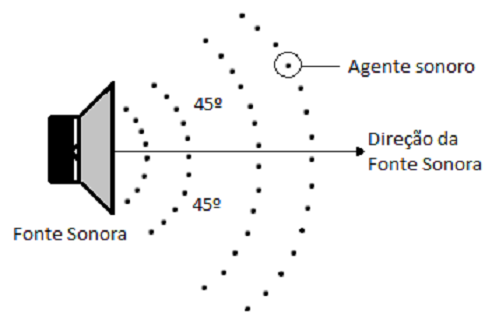
\includegraphics[scale=0.55]{figuras/fonte_sonora}
\caption{Fonte Sonora}
\label{fonte_sonora}
\end{figure}

A fonte sonora lança cada agente em uma determinada direção. A potência na qual a fonte sonora emite os agentes pode ser configurada. Após o agente sonoro ser emitido pela fonte, ele seguirá na direção em que foi lançado até encontrar um obstáculo, onde então, irá recalcular sua intensidade sonora com base no índice de absorção do material do obstáculo encontrado, e irá alterar também sua direção com base no ângulo de inclinação do obstáculo. A cada reflexão, os agentes sonoros vão perdendo potência devido ao coeficiente de absorção sonora do material que reveste o obstáculo, até atingir uma intensidade sonora considerada inaudível ao ouvido humano.

Nesta prova de conceito, foram consideradas apenas duas dimensões para a representação simplificada do sistema, sendo assim, o som se desloca em um plano 2D e os obstáculos são definidos por linhas, conforme o exemplo de ambiente ilustrado na figura \ref{ambiente}.

\FloatBarrier 
\begin{figure}[!htb]
\centering
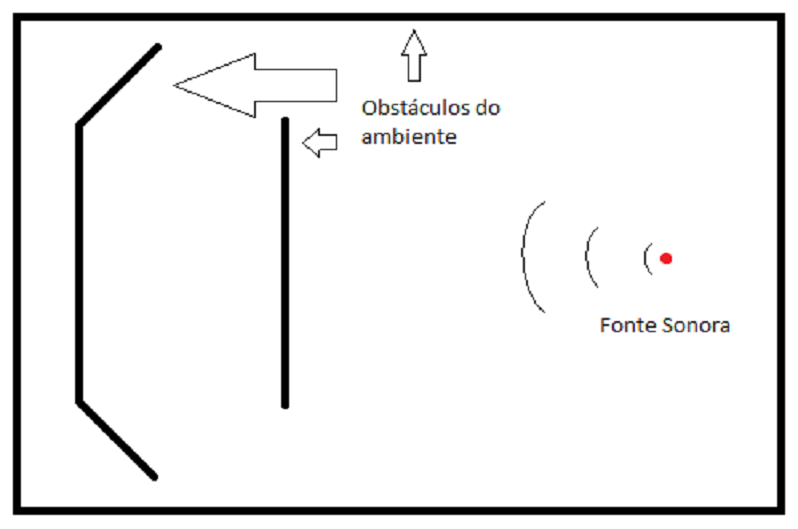
\includegraphics[scale=0.55]{figuras/ambiente}
\caption{Ambiente bidimensional}
\label{ambiente}
\end{figure}

O comportamento dos agentes foi acompanhado a partir do JADE GUI, ferramenta gráfica nativa do JADE para acompanhamento dos agentes e suas trocas de mensagens. A figura \ref{jade_gui} ilustra esta ferramenta. 

\FloatBarrier 
\begin{figure}[!htb]
\centering
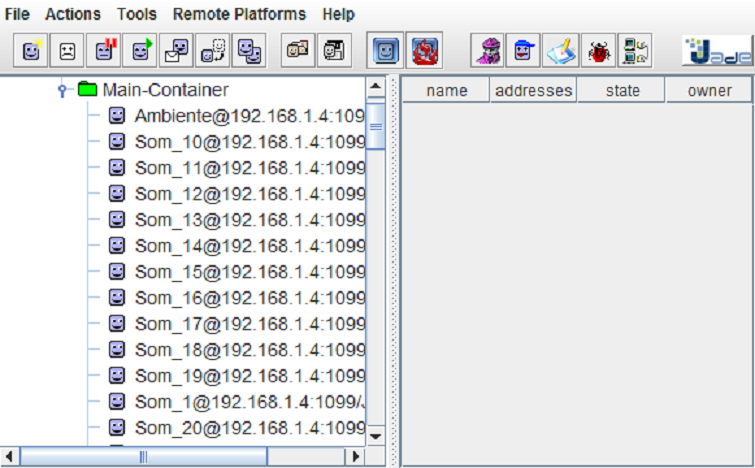
\includegraphics[scale=0.55]{figuras/jade_gui}
\caption{JADE GUI}
\label{jade_gui}
\end{figure}

Nesta abordagem híbrida para a solução da prova de conceito, o agente som se torna responsável por conhecer os obstáculos presentes no ambiente no qual está inserido, pois os obstáculos não participam ativamente do sistema, ou seja, não são capazes de realizar trocas de mensagens com os agentes. Como o ambiente é o agente que conhece todos os elementos presentes na sala, ele é responsável por informar à fonte sonora como estão mapeados os obstáculos dentro do ambiente. Dessa forma, quando a fonte sonora lança um pulso, ela é responsável por passar a cada agente sonoro essa informação no momento de sua criação.

\subsection{Refinamento da proposta}

Após a implementação da prova de conceito seguindo o modelo híbrido, onde os obstáculos são objetos e os demais elementos são agentes, foi possível trabalhar com um volume de até 447 agentes sonoros, ou seja, um agente a cada 0,2º considerando uma fonte com abertura de 90º, de forma segura, sem causar travamento do sistema e nem prejudicar a comunicação dos agentes. Porém, a velocidade da simulação cai significativamente, levando 3 minutos e 29 segundos até o final do último som no ambiente. Com um volume de 181 agentes, basicamente um agente a cada 0,5º em uma fonte sonora com abertura de 90º, foi possível realizar a simulação a um tempo de 1 minuto e 24 segundos. Ambos os resultados foram mais satisfatórios que a proposta inicial do sistema totalmente baseada em multiagentes, não apenas pelo tempo, mas também pelo fato de a primeira proposta não suportar um volume maior que 91 agentes sem apresentar problemas na troca de mensagens, ocasionando um erro associado à identificação de colisão dos agentes com os obstáculos.

Vale ressaltar que as configurações de máquina utilizadas nessa simulação não são ideais. Sistemas multiagentes são intrinsecamente distribuídos e para obter melhores resultados em termos de desempenho, seria necessário utilizar mais de uma máquina. Entretanto, tal recurso não foi viável durante a condução do experimento.


\section[O simulador acústico]{O simulador acústico}

Esta seção trata de aspectos do simulador acústico desenvolvido neste trabalho, tais como, arquitetura, como realizar uma simulação dentro do sistema e as devidas verificações e validações realizadas no mesmo.

\subsection{Descrição do simulador}

A partir do referencial bibliográfico estudado neste trabalho e da prova de conceito desenvolvida no decorrer do TCC 01, foi possível definir que o simulador, objeto de estudo deste trabalho, consiste em um sistema que seja capaz de representar o comportamento sonoro dentro de um ambiente através de agentes de software, que sejam capazes de interagir de forma autônoma com os elementos do ambiente representados no sistema.

Com base na simulação realizada na prova de conceito, foi possível identificar que, por questões de desempenho, a solução do sistema final deveria ser composta por pelo menos dois paradigmas, o paradigma orientado a objetos e o de sistemas multiagentes.

Para a solução final, o sistema foi evoluído a fim de apresentar graficamente o andamento da simulação e o comportamento do som dentro do ambiente. O comportamento dos agentes sonoros também foi aprimorado. O nível de intensidade sonora no ambiente cai a medida que o som percorre o ambiente e sofre colisões com os obstáculos presentes, considerando uma taxa de decaimento em um ambiente tridimensional, mesmo a visualização da simulação sendo bidimensional. Tal contexto permite calcular o tempo de reverberação no ambiente considerando o parâmetro RT60, que representa o tempo em que o nível de intensidade sonora em um ambiente diminui em 60dB \cite{loschi}.

Tanto os agentes quanto os objetos do sistema foram escritos na linguagem de programação Java. A ferramenta utilizada para controle de versão é o Git, juntamente com o repositório GitHub, afim de promover a cultura de software livre e abrir espaço para a comunidade que deseja contribuir ou estudar sobre o assunto.

\subsection{Arquitetura}

Este simulador foi desenvolvido com base no modelo de arquitetura em camadas, onde temos duas camadas principais: apresentação e negócio. A camada de apresentação é responsável pela interface com o usuário. Nesta camada estão situados todos os componentes gráficos do sistema. Tais componentes foram desenvolvidos utilizando o pacote Swing do Java, juntamente com a biblioteca JFreeChart para plotagem dos gráficos. 

Já a camada de negócio compreende a máquina de raciocínio deste simulador, onde estão situados os agentes e os objetos que atuam nas principais funcionalidades do sistema. Toda essa camada foi desenvolvida utilizando a linguagem de programação Java. Os agentes de software foram implementados com o apoio do \textit{framework} JADE. A figura \ref{arquitetura_geral} ilustra o modelo de arquitetura em camadas descrito.

\FloatBarrier 
\begin{figure}[!htb]
\centering
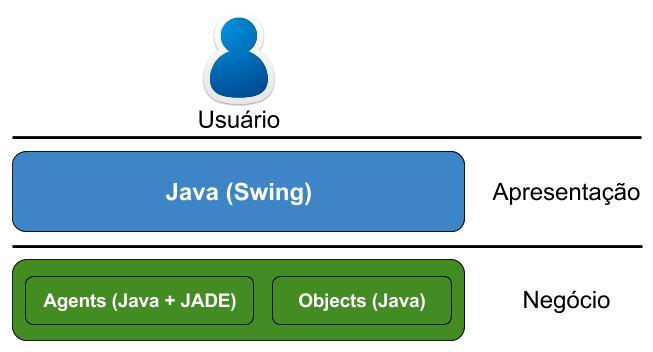
\includegraphics[scale=0.55]{figuras/arquitetura_geral}
\caption{Arquitetura visão geral}
\label{arquitetura_geral}
\end{figure}

Dada a camada de negócio, o sistema é composto por três tipos de agentes, sendo eles, ambiente, fonte sonora e sons. Cada um possui um objeto correspondente, onde estão implementados os métodos que irão compor seus comportamentos. Outro elemento do sistema é o obstáculo, porém, este deixou de ser um agente, sendo tratado, no momento, como objeto também. 

O Ambiente é o agente responsável pela criação das fontes sonoras que, por sua vez, são responsáveis pela criação dos sons. Cada um desses agentes possui um objeto relacionado, por exemplo, para criar um agente do tipo \textit{SoundAgent}, é necessário passar um objeto do tipo \textit{Sound} como argumento, assim como é preciso passar um objeto do tipo \textit{SoundSource} para criar um agente do tipo \textit{SoundSourceAgent}. Esses objetos são responsáveis por armazenar os valores dos atributos do agente correspondente e implementar os métodos que irão compor seus comportamentos.

Outro elemento importante para se realizar uma simulação é o obstáculo. A classe \textit{Obstacle}, possui os atributos e métodos necessários para instanciar um objeto do tipo, como por exemplo, o índice de absorção, que por sua vez, será consultado toda vez que um agente sonoro colidir com o obstáculo. Este índice é importante para que o agente som possa calcular sua intensidade sonora após uma colisão, pois parte da sua energia será absorvida pelo obstáculo. O índice de absorção de um material varia de acordo com a frequência em que o som se encontra no momento da colisão. A classe \textit{Obstacle} também é responsável por manter um \textit{HashMap} com todos os obstáculos criados e seus respectivos IDs, para que os agentes possam consultá-los quando necessário.

O modelo da arquitetura dessa máquina de raciocínio está ilustrado na figura \ref{arquitetura}.

\begin{figure}[!htb]
\centering
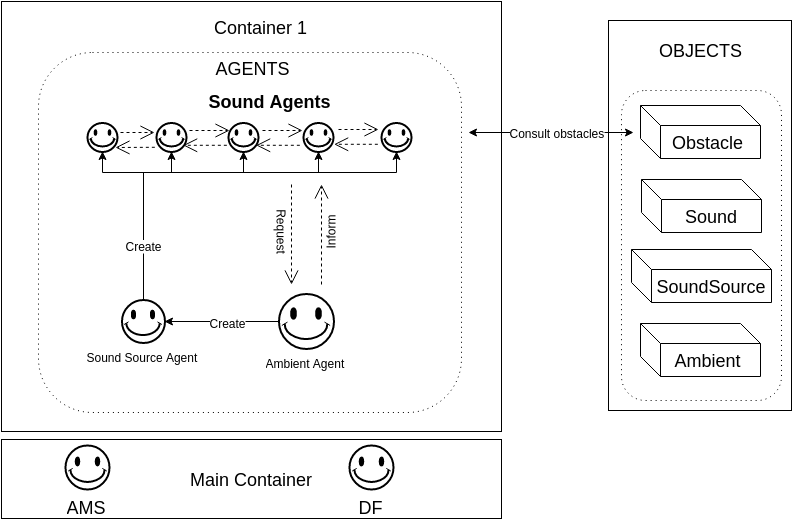
\includegraphics[scale=0.4]{figuras/arquitetura}
\caption{Arquitetura da máquina de raciocínio do Simulador Acústico}
\label{arquitetura}
\end{figure}

Além da arquitetura base do sistema, também é implementada em uma camada transversal a todo o sistema, correspondente à arquitetura do \textit{framework} JADE\footnote{\url{http://jade.tilab.com/}}. O JADE é utilizado para a implementação dos agentes neste projeto, provendo funcionalidades na camada de \textit{middleware}. Este \textit{framework} é interoperável, permitindo a comunicação entre agentes JADE e outros tipos de agentes fora da plataforma. 

O JADE faz uso da abstração de \textit{containers}, nos quais estão os agentes. Agentes podem ou não estar distribuídos na rede, sendo que cada \textit{container} pode conter um ou mais agentes. Esta plataforma deve conter obrigatoriamente o \textit{Main Container}, um \textit{container} responsável pelo gerenciamento de agentes, composto pelos agentes AMS e DF. O AMS (Agent Management System) é único na plataforma e é responsável por conhecer todos os agentes presentes no sistema, pois é ele quem exerce o controle sobre o acesso e o uso da plataforma, além de manter  a lista de identificadores dos agentes (AID). Portanto, todos os agentes criados devem ser registrados no AMS. 

Já o agente DF (Directory Facilitator), oferece todas as interações básicas da plataforma, além de oferecer um conjunto de métodos para a implementação do comportamento do agente. Nem todos os agentes são registrados no DF, apenas aqueles que prestam algum serviço. O modelo da arquitetura do JADE pode ser visualizado na figura \ref{jade}.

\begin{figure}[!htb]
\centering
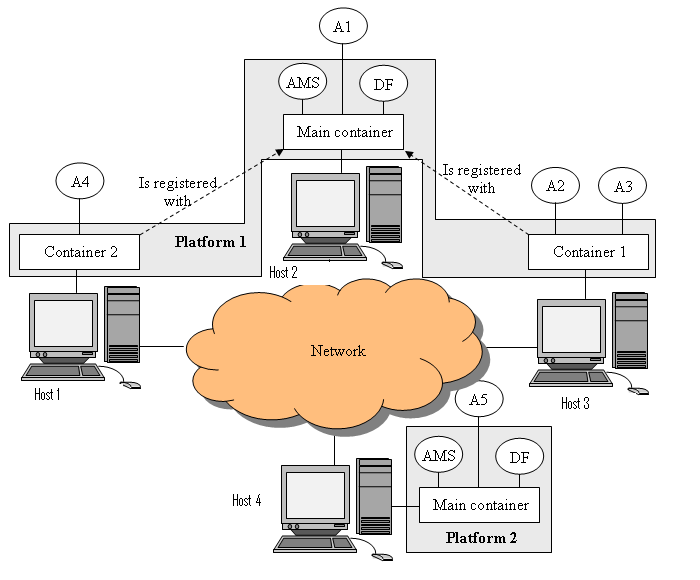
\includegraphics[scale=0.5]{figuras/jade}
\caption{Arquitetura JADE$ ^{1} $}
\label{jade}
\end{figure}

Os Agentes JADE possuem um ciclo de vida, conforme ilustrado na figura \ref{ciclo_jade}. O primeiro passo desse ciclo de vida é a criação do agente, seguido de sua inicialização. Ao ser inicializado o agente se torna ativo para execução de tarefas ou comportamentos, podendo ser suspenso e retornar ao estado de ativo posteriormente. Os agentes também podem entrar em modo de espera em busca de algum recurso que outro agente está executando, e retornar quando este recurso for liberado. Outro estado é quando o agente está em trânsito, se movimentando pela rede, porém, independente do estado em que o agente esteja, ele pode ser destruído.

\begin{figure}[!htb]
\centering
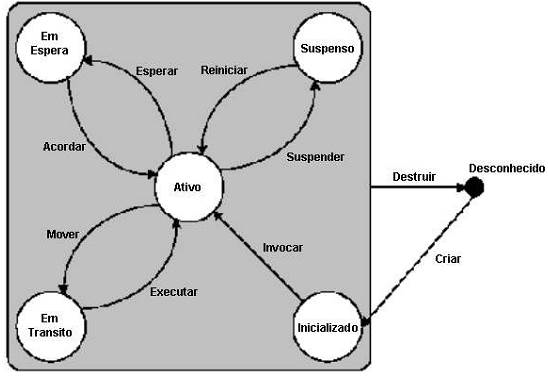
\includegraphics[scale=0.7]{figuras/ciclo_de_vida_agente_jade}
\caption{Ciclo de vida do agente JADE \cite{leonardo}}
\label{ciclo_jade}
\end{figure}

A estrutura dos pacotes deste simulador pode ser visualizada na figura \ref{pacotes}.

\begin{figure}[!htb]
\centering
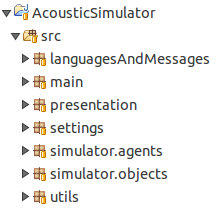
\includegraphics[scale=0.8]{figuras/pacotes}
\caption{Estrutura de pacotes do simulador acústico}
\label{pacotes}
\end{figure}

\pagebreak

\subsection{Realizando uma simulação}

Esta seção evidencia como utilizar o simulador acústico. O usuário pode definir um ambiente e suas dimensões, assim como inserir obstáculos e fontes sonoras dentro dele. Também é possível que o usuário inicie, pause, retome ou encerre uma simulação a qualquer momento.

O código do simulador acústico é aberto e está disponível no
GitHub\footnote{\url{https://github.com/gabriel-augusto/AcousticSimulator}}.

\subsubsection{Tela inicial do simulador}

Ao iniciar o simulador acústico, irá aparecer a tela principal do sistema, onde está localizada a maior parte de suas funcionalidades. No canto superior esquerdo, é possível observar o menu, com as opções \textit{action} e \textit{edit}, assim como a barra de ferramentas do sistema. Logo abaixo, na tela, é possível visualizar o espaço para as tabelas de obstáculos e fontes sonoras da simulação. À direita, o espaço para visualizar a simulação em andamento, conforme é evidenciado na figura \ref{tela_inicial}.

\begin{figure}[!htb]
\centering
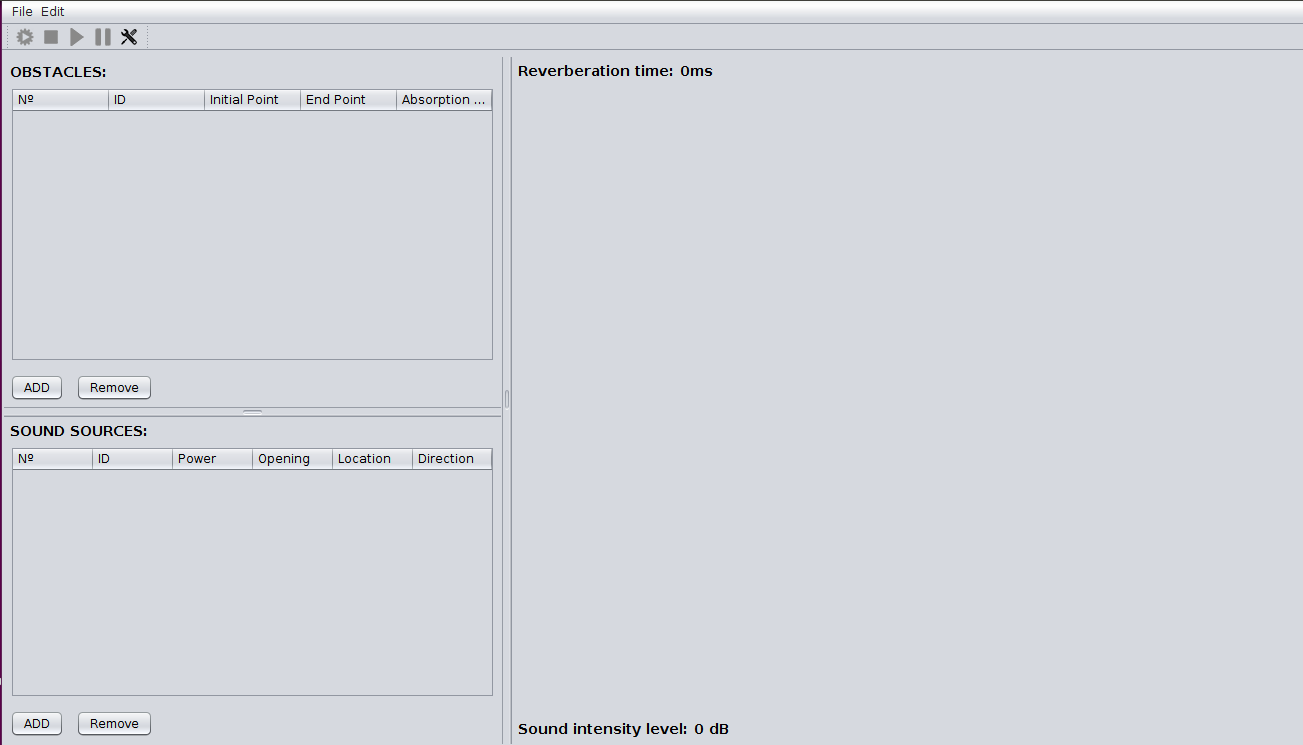
\includegraphics[scale=0.35]{figuras/telas/tela_inicial}
\caption{Tela inicial do simulador acústico}
\label{tela_inicial}
\end{figure}

\subsubsection{Adicionando obstáculos}

O primeiro passo ao realizar uma simulação consiste em adicionar os obstáculos que irão compor o ambiente. Cada obstáculo possui um ponto inicial, um ponto final e um índice de absorção associado.

Há duas formas de inserir obstáculos. A primeira delas é informar o índice de absorção e as dimensões do ambiente. Após informar as dimensões, o software cria quatro obstáculos com o índice de absorção especificado compondo as delimitações do ambiente. Para utilizar este recurso, basta clicar no menu "Edit -> Define Ambient" ou utilizar as teclas de atalho "Ctrl+D" e informar os dados ao sistema na tela de configuração do ambiente que está evidenciada na figura \ref{ambient_settings}.

\begin{figure}[!htb]
\centering
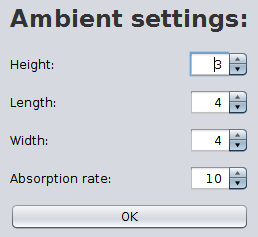
\includegraphics[scale=0.6]{figuras/telas/ambient_settings}
\caption{Tela de configuração do ambiente}
\label{ambient_settings}
\end{figure}

Outra forma de se adicionar obstáculos ao ambiente, é inseri-los individualmente. Para isto, basta clicar no menu "Edit -> Add Obstacle" ou clicar no botão "ADD" abaixo da tabela de obstáculos.

Para definir um obstáculo, é necessário informar as coordenadas do seu ponto inicial e final, assim como seu respectivo índice de absorção na tela de criação de obstáculos, evidenciada na figura \ref{add_obstacle}. Dessa forma, o sistema irá criar um obstáculo em forma de linha reta dentro do seu ambiente. Vale ressaltar que, apesar da máquina de raciocínio do simulador estar preparada para trabalhar com diversos obstáculos, devido ao uso da biblioteca de gráficos JFreeChart, não foi possível plotar esses obstáculos dentro do ambiente, uma vez que eles são representados como linhas retas e os sons são representados como pontos.

\begin{figure}[!htb]
\centering
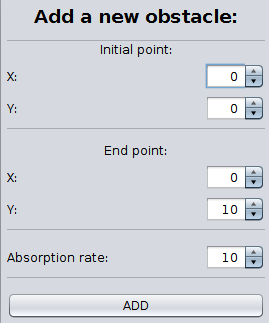
\includegraphics[scale=0.6]{figuras/telas/add_obstacle}
\caption{Tela de criação de obstáculos}
\label{add_obstacle}
\end{figure}

Todos os obstáculos criados, assim como seus respectivos parâmetros, podem ser visualizados na tabela de obstáculos na tela principal do sistema, a qual está evidenciada na figura \ref{tabela_obstaculos}. Abaixo desta tabela, há dois botões com as opções de adicionar e remover, permitindo realizar estas ações de forma rápida e prática. Para remover um obstáculo do ambiente, basta selecioná-lo na tabela de obstáculos e clicar no botão remover.

\begin{figure}[!htb]
\centering
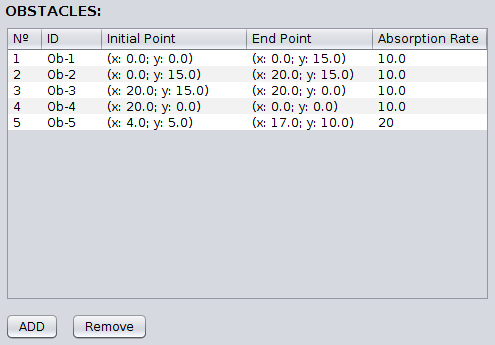
\includegraphics[scale=0.6]{figuras/telas/obstacles_table}
\caption{Tabela de obstáculos}
\label{tabela_obstaculos}
\end{figure}

\subsubsection{Adicionando fontes sonoras}

Após definir as delimitações do ambiente e seus obstáculos, é o momento de inserir uma ou mais fontes sonoras. Para realizar uma simulação, é necessário ter no mínimo uma fonte sonora dentro do ambiente.

Existem três maneiras de abrir a tela de configurações da fonte sonora. Essa tela está ilustrada na figura \ref{sound_source_screen}. A primeira delas é através do menu "Edit -> Add Sound Source". Esta tela também pode ser acessada através do botão "ADD", abaixo da tabela de fontes sonoras, ou através das teclas de atalho "Ctrl + H".

As configurações de uma fonte sonora incluem seu ângulo de abertura em graus, suas coordenadas dentro do ambiente, a direção para a qual está apontada e o número de agentes sonoros que serão emitidos pela fonte. O número de agentes sonoros reflete na precisão da simulação, ou seja, quanto mais agentes sonoros são emitidos, mais fiel se torna o resultado da simulação. Entretanto, um número maior de agentes requer mais recursos computacionais.

\begin{figure}[!htb]
\centering
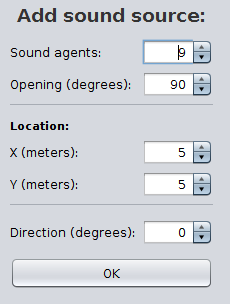
\includegraphics[scale=0.6]{figuras/telas/add_sound_source}
\caption{Tela de configuração da fonte sonora}
\label{sound_source_screen}
\end{figure}

Igualmente aos obstáculos, todas as fontes sonoras criadas, assim como seus respectivos parâmetros, podem ser visualizados na tabela de fontes sonoras na tela principal do sistema, conforme ilustrado na figura \ref{tabela_fs}. Esta tabela é bastante parecida com a tabela de obstáculos, contendo os dois botões com as opções de adicionar e remover, permitindo realizar estas ações de forma rápida e prática. Para remover uma fonte sonora do ambiente, basta selecioná-la na tabela de fontes sonoras e clicar no botão remover.

\begin{figure}[!htb]
\centering
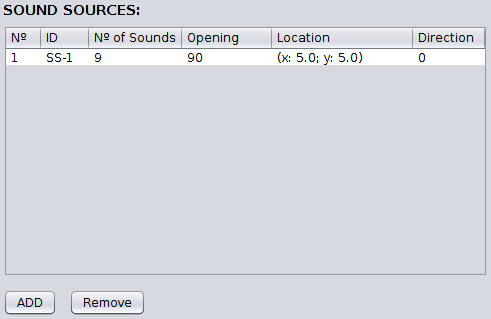
\includegraphics[scale=0.6]{figuras/telas/ss_table}
\caption{Tabela de fontes sonoras}
\label{tabela_fs}
\end{figure}

\subsubsection{Configurando a velocidade da simulação}

A velocidade da simulação representa o tempo em que a posição dos agentes sonoros é atualizada. Para configurar essa velocidade, é necessário acessar a tela de configurações da simulação, evidenciada na figura \ref{settings}, através do menu "edit -> simulation settings" ou através do ícone "Simulation Settings" na barra de ferramentas. As teclas de atalho para acessar essa tela são "Ctrl + I".

\begin{figure}[!htb]
\centering
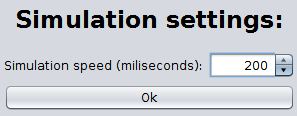
\includegraphics[scale=0.6]{figuras/telas/simulation_settings}
\caption{Tela de configurações da simulação}
\label{settings}
\end{figure}

\subsubsection{Executando uma simulação}

Após definir as dimensões do ambiente, inserir os obstáculos e fontes sonoras e configurar a velocidade, é possível executar a simulação. Com todos os itens configurados, há três maneiras de executar uma simulação. A primeira delas é através do menu "Action -> run simulation". Outra opção é através do ícone "Run simulation", na barra de ferramentas e por essa opção estar localizada diretamente na tela inicial do sistema, ela pode ser acessada de forma mais fácil e intuitiva. Há também a possibilidade de executar a simulação através das teclas de atalho "Ctrl + R".

Com a simulação em execução, é possível pausar, resumir ou encerrar a simulação à qualquer momento de sua execução. Todas essas opções estão disponíveis no menu "Action" ou na barra de ferramentas do sistema que está evidenciada na figura \ref{toolbar}.

\begin{figure}[!htb]
\centering

\includegraphics[scale=0.6]{figuras/telas/toolbar}
\caption{Barra de ferramentas}
\label{toolbar}
\end{figure}

Durante a execução da simulação, é possível visualizar o comportamento do som dentro do ambiente na tela inicial do sistema, conforme evidenciado na figura \ref{simulation}. Os sons são representados graficamente por pontos azuis, enquanto as fontes sonoras são representadas por pequenos quadrados verdes.

\begin{figure}[!htb]
\centering
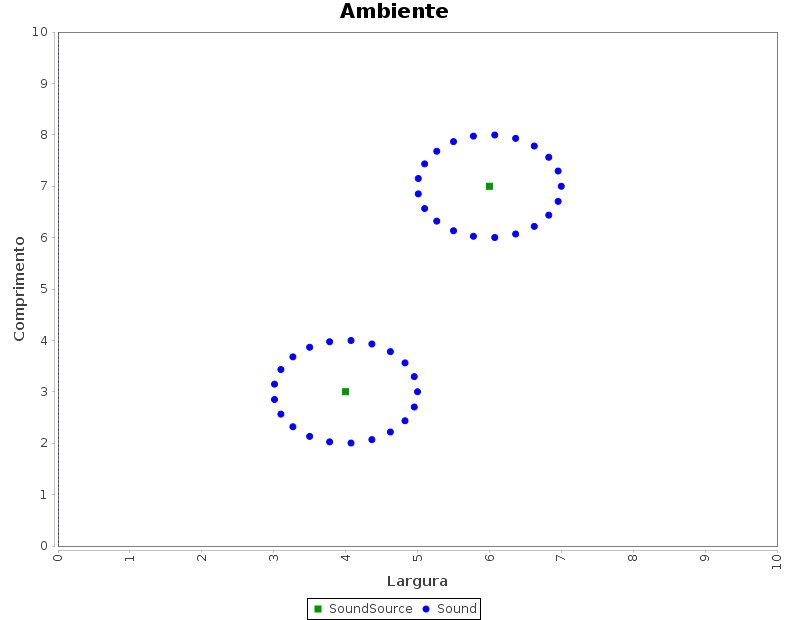
\includegraphics[scale=0.4]{figuras/telas/simulation3}
\caption{Visualização gráfica da simulação em andamento.}
\label{simulation}
\end{figure}

Ao fim da simulação, o campo com o valor do tempo de reverberação, localizado acima do espaço destinado ao acompanhamento da simulação, é atualizado, apresentando então, o tempo de reverberação do ambiente configurado.

\subsection{Testes unitários e cobertura de código}

Pra realização dos testes unitários e análise de cobertura de código fonte, foram adotadas as ferramentas JUnit\footnote{\url{http://junit.org/}} e EclEmma\footnote{\url{http://eclemma.org/}} respectivamente. Devido ao fato de os agentes comportamentais não possuirem uma ferramenta de validação comportamental adequada até o presente momento, foram criados objetos relacionados a cada um dos agentes, onde todas as rotinas utilizadas pelos comportamentos dos agentes foram migradas para seus respectivos objetos. Dessa forma, foi possível testar as rotinas utilizando as ferramentas adotadas. Porém, os agentes em si não puderam ser completamente testados.

Devido ao fato de não haver uma ferramenta de validação adequada para agentes comportamentais, foi estabelecida uma meta de 80\% de cobertura de testes. O quadro com a cobertura de testes pode ser visualizado na figura \ref{cobertura}. Como é possível observar, a cobertura esperada foi alcançada.

\begin{figure}[!htb]
\centering
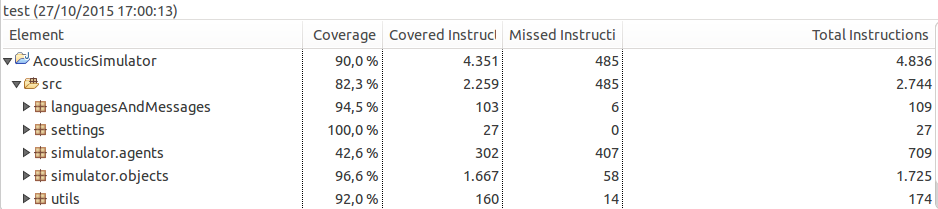
\includegraphics[scale=0.45]{figuras/cobertura}
\caption{Cobertura de código.}
\label{cobertura}
\end{figure}

\subsection{Métricas de qualidade de código fonte}

Esta seção evidencia o resultado da qualidade do código fonte do simulador desenvolvido durante esse trabalho. Através da análise estática de código fonte foi possível obter métricas referentes ao código do simulador e realizar uma análise qualitativa dos resultados obtidos. A ferramenta adotada para realizar a análise foi a Analizo\footnote{\url{http://www.analizo.org/}}

Segundo \citeonline{kalibro}, medir e monitorar a qualidade do software é fundamental, independente da metodologia adotada para o desenvolvimento. Mesmo uma ótima bateria de testes pode produzir informações apenas sobre características externas, não refletindo qualidades como manutenibilidade, modularidade, flexibilidade e simplicidade \cite{kalibro}.

Para realizar a análise estática do código, foram utilizadas as métricas e seus respectivos valores de referência baseados na dissertação de \citeonline{kalibro}. Tais valores foram obtidos baseando-se nos resultados da análise de um ou mais "projetos
modelo", analisados no Capítulo 4 da tese de \citeonline{meirelles}.

Dentre as métricas suportadas pelo Analizo, \citeonline{meirelles} seleciona um subconjunto representativo, pois foi constatado que muitas delas eram redundantes por medir prioridades muito correlacionadas. As métricas selecionadas abrangem diversos aspectos de uma classe:

\begin{enumerate}
\item Conexões aferentes, ou ACC, uma medida de acoplamento.
\item Média da complexidade ciclomática dos métodos, ou ACCM.
\item Média do tamanho dos métodos, ou AMLOC.
\item Média do número de parâmetros por método, ou ANPM.
\item Profundidade na árvore de herança, ou DIT.
\item Número de métodos, ou NOM.
\item Número de atributos públicos, ou NPA.
\item Complexidade estrutural, ou SC, uma medida que combina acoplamento (CBO) e coesão (LCOM4).
\end{enumerate}

A figura \ref{analise} apresenta os resultados da análise estática realizada. É possível observar que todos os valores ficaram entre bom e ótimo, segundo os intervalos sugeridos por \citeonline{kalibro}. Devido a esses resultados, e as atividades contínuas de refatoração durante o desenvolvimento do simulador, não foi realizada outra refatoração após a análise estática do código fonte.

\begin{figure}[!htb]
\centering
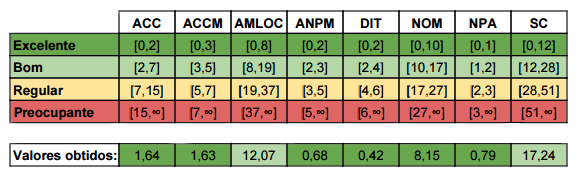
\includegraphics[scale=0.6]{figuras/Analise_estatica}
\caption{Análise estática do código fonte.}
\label{analise}
\end{figure}

\subsection{Comparação entre os cenários de uso avaliados}

Para validar se os resultados gerados pelas simulações realizadas pelo simulador acústico desenvolvido neste trabalho estavam de acordo com o esperado, foram coletados os dados de mais dois simuladores que calculam o tempo de reverberação do ambiente através de seus parâmetros. Para que a comparação com o simulador acústico desenvolvido fosse possível, era necessário que o simulador a ser comparado permitisse a visualização dos coeficientes de absorção dos materiais que ele disponibiliza, pois qualquer diferença nesses coeficientes, implica em uma diferença considerável no resultado final da simulação. Este fato restringiu bastante a possibilidade de comparação com diversas ferramentas disponíveis no mercado.

Por fim, foram encontradas duas ferramentas que permitem visualizar os coeficientes de absorção de seus materiais ou a média final dos coeficientes de absorção adotados. A primeira delas é a ferramenta de cálculo de tempo de reverberação da hyperphysics\footnote{\url{http://hyperphysics.phy-astr.gsu.edu/}}. Esta ferramenta permite editar manualmente os coeficientes de absorção de cada um dos obstáculos adicionados, possibilitando realizar a simulação com parâmetros completamente idênticos. A segunda é a rt60calc\footnote{\url{http://www.belgi.net/audiocorp/techinfo/rt60calc.htm}} da Belgi. Esta ferramenta, apesar de não permitir informar o valor dos coeficientes de absorção diretamente, permite inserir os materiais desejados e informa o coeficiente médio ao final, possibilitando atingir manipular os materiais disponíveis e atingir valores bem próximos. Ambas as ferramentas foram adotadas para serem usadas nas comparações.

As especificações técnicas da máquina, a qual foi utilizada para a realização da comparação entre os cenários de uso levantados foram: um processador Intel Core i7, modelo 2630QM de 2Ghz e uma memória RAM de 6Gb. O sistema operacional utilizado foi o Ubuntu,
versão 14.04.3 LTS de 64 bits e a versão do Java utilizada foi a "1.8.0\_66".

Para realizar as comparações, foram criados três cenários, o primeiro foi um ambiente com 4m de largura, 4m de comprimento e 3m de altura. Para o segundo cenário, foi especificado um ambiente um pouco maior, possuindo 3m de largura, 7m de comprimento e 4m de altura. Por fim, para o último cenário foi especificado um ambiente bem maior, possuindo 25m de largura, 20m de comprimento e 6m de altura. O coeficiente médio de absorção foi de 20\% para todos os cenários. Essas configurações podem ser vistas na tabela \ref{cenarios}. 

\begin{table}[]
\centering
\caption{Cenários avaliados}
\label{cenarios}
\begin{tabular}{|l|c|c|c|}
\hline
\textbf{Dados do ambiente} & \multicolumn{1}{l|}{\textbf{Cenário 1}} & \multicolumn{1}{l|}{\textbf{Cenário 2}} & \multicolumn{1}{l|}{\textbf{Cenário 3}} \\ \hline
Largura              & 4 m                  & 3 m                & 25 m            \\
Comprimento          & 4 m                  & 7 m                & 20 m            \\
Altura               & 3 m                  & 4 m                & 6  m            \\
Absorção média       & 9 \%                 & 10 \%              & 20 \%           \\ \hline
\end{tabular}
\end{table}

Após especificar os cenários a serem analisados em cada uma das ferramentas, foi realizada a simulação em cada um delas. Após a realização da simulação, os dados referentes ao tempo de reverberação foram coletados. Os resultados podem ser visualizados na tabela \ref{resultados}.

\begin{table}[]
\centering
\caption{Resultados das simulações}
\label{resultados}
\begin{tabular}{|l|c|c|c|}
\hline
\textbf{Ferramenta} & \textbf{Cenário 1} & \textbf{Cenário 2} & \textbf{Cenário 3} \\ \hline
Acoustic Simulator  & 1073 ms             & 1109 ms             & 1568 ms            \\
belgi rt60calc      & 1070 ms             & 1106 ms             & 1563 ms            \\
hyperphysics        & 1073 ms             & 1108 ms             & 1568 ms            \\ \hline
\end{tabular}
\end{table}

Os resultados das simulações nos três cenários foram bem próximos. O gráfico da figura \ref{comparacao} demonstra a proximidade entre os tempos de reverberação entre as ferramentas para cada um dos cenários avaliados nessa comparação. Para afirmar tal proximidade, foi calculado o coeficiente de variação, medida de dispersão que representa a homogneidade entre os dados coletados expressa pela seguinte equação: $ cv = 100\frac{\sigma}{\mu} $, onde cv é o coeficiente de variação, $\sigma$ é o desvio padrão e $\mu$ é a média.

\begin{figure}[!htb]
\centering
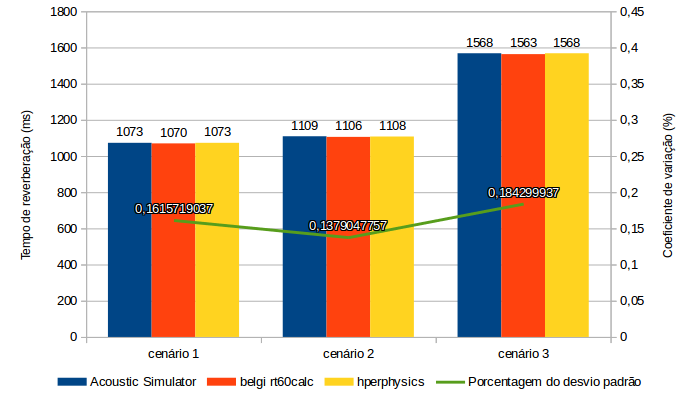
\includegraphics[scale=0.6]{figuras/comparacao}
\caption{Tempo de reverberação dos simuladores por cenário.}
\label{comparacao}
\end{figure}

Considerando os valores obtidos para o coeficiente de variação, foi possível concluir que a dispersão entre os valores dos simuladores é mínima, incluindo o simulador acústico desenvolvido neste trabalho, uma vez que todos os valores ficaram abiaxo de 1\%. Sendo assim, os valores de tempo de reverberação obtidos pelo simulador acústico desenvolvido neste trabalho (i.e. Acoustic Simulator), estão dentro do esperado.

\section{Considerações finais}

A proposta deste sistema consiste em um sistema de simulação acústica capaz de representar um ambiente e, a partir deste sistema, por meio de uma fonte sonora, emitir agentes sonoros capazes de interagir com os elementos presentes no ambiente até que o nível de intensidade sonora dentro do ambiente caia em 60dB, onde então o som é caracterizado como finalizado e o agente é destruído. O parâmetro que simboliza o tempo de reverberação no ambiente, considerando essa redução do nível de intensidade sonora do ambiente em 60db, é denominado RT60.

A máquina de raciocínio deste sistema foi construída utilizando a linguagem de programação Java e é baseada na arquitetura de agentes de software, utilizando recursos como a troca de mensagens, assincronismo e autonomia. Porém, para que isto fosse possível, o sistema precisou rodar por cima da arquitetura do \textit{framework} JADE. Trata-se de uma ferramenta escolhida para a implementação dos agentes deste simulador. Adicionalmente, a camada de apresentação do simulador foi implementada utilizando o pacote Swing do Java juntamente com a biblioteca JFreeChart, para a criação dos gráficos em 2D.

Quanto aos testes, foram realizados testes de unidade para validar os módulos do sistema, onde o nível de cobertura adotado foi de 80\%. Afim de verificar a qualidade do código fonte, foi utilizada a ferramenta Analizo para a coleta de métricas de código fonte. As métricas consideradas foram: ACC, ACCM, AMLOC, ANPM, DIT, NOM, NPA e SC. Tais métricas foram escolhidas com o intuito de evitar redundância entre as métricas suportadas pela ferramenta Analizo, segundo o estudo de \citeonline{kalibro}.

Pra analizar os resultados finais obtidos pelas simulações do simulador desenvolvido neste trabalho, foram feitas comparações em três cenários diferentes com as ferramentas rt60calc e hyperphysics. A proximidade entre os valores da simulação foi analisada considerando o coeficiente de variação entre eles, onde todos os coeficientes ficaram abaixo de 0,2\%, sendo então, considerados aceitáveis os resultados obtidos pelo simulador. 

Todo o controle de versão é feito a partir do git e está disponível de forma livre no repositório do GitHub\footnote{\url{https://github.com/gabriel-augusto/AcousticSimulator}}, sendo possível acompanhar todo o desenvolvimento do simulador e contribuir com a comunidade de software livre.